\documentclass{article}
\usepackage{tikz}
\usepackage{array}
\usetikzlibrary{arrows.meta}
\usepackage{booktabs}
\def\x{1}
\def\y{1}
% Define column type for centered text with specified width
\newcolumntype{C}[1]{>{\centering\arraybackslash}p{#1}}
\begin{document}
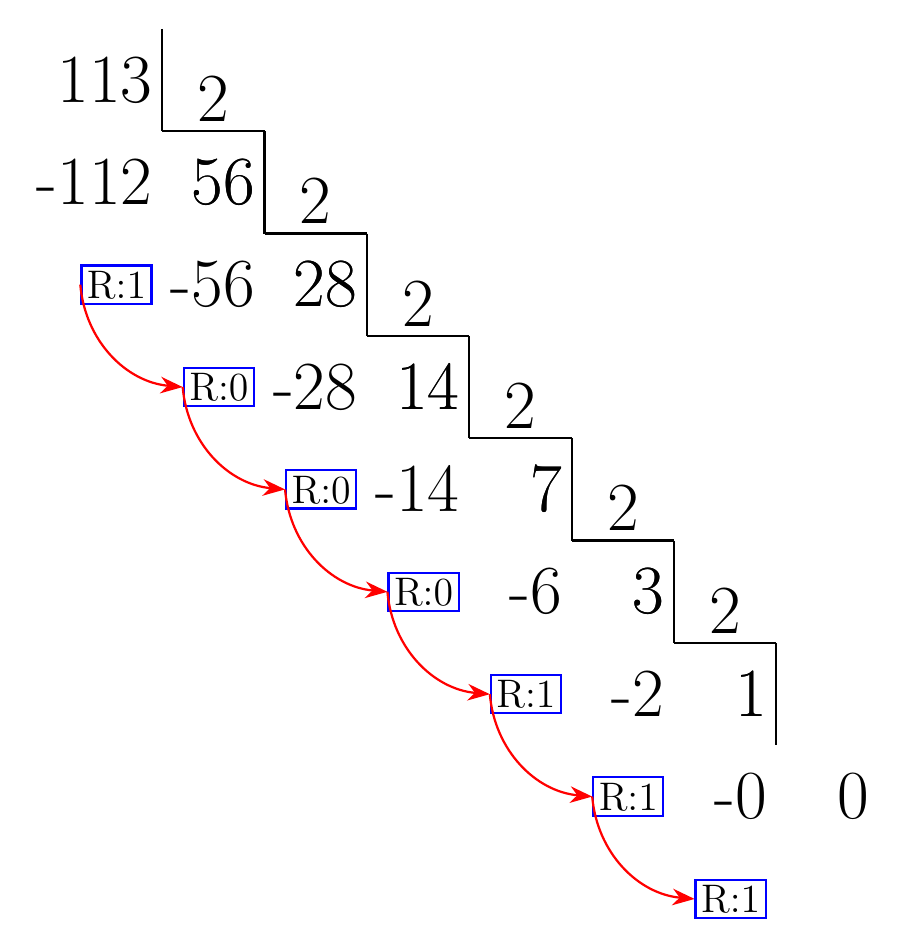
\begin{tikzpicture}[scale=1.3]
    % Ladder pattern: vertical down, horizontal right, vertical down, horizontal right, etc.
    \draw[thick] (0,4) -- (0,3);        % vertical down
    \node[left] at (0,3.5) {\Huge 113};)
    \node[left] at (0,2.5) {\Huge -112};)
    \node[right, draw=blue, thick, inner sep=2pt] at (0.2-\x,2.5-\y) {\Large R:1};)
    \draw[thick] (0,3) -- (1,3);        % horizontal right
    \node[above] at (0.5,3) {\Huge 2};
    \node[left] at (1,2.5) {\Huge 56};)
    \draw[thick] (1,3) -- (1,2);        % vertical down
    \node[left] at (1,2.5) {\Huge 56};)
    \node[left] at (1,1.5) {\Huge -56};)
    \node[right, draw=blue, thick, inner sep=2pt] at (1.2-\x,1.5-\y) {\Large R:0};)
    \draw[thick] (1,2) -- (2,2);        % horizontal right
    \node[above] at (1.5,2) {\Huge 2};
    \node[left] at (2,1.5) {\Huge 28};)
    \draw[thick] (2,2) -- (2,1);        % vertical down
    \node[left] at (2,1.5) {\Huge 28};)
    \node[left] at (2,0.5) {\Huge -28};)
    \node[right, draw=blue, thick, inner sep=2pt] at (2.2-\x,0.5-\y) {\Large R:0};)
    \draw[thick] (2,1) -- (3,1);        % horizontal right
    \node[above] at (2.5,1) {\Huge 2};
    \node[left] at (3,0.5) {\Huge 14};)
    \draw[thick] (3,1) -- (3,0);        % vertical down
    \node[left] at (3,0.5) {\Huge 14};)
    \node[left] at (3,-0.5) {\Huge -14};)
    \node[right, draw=blue, thick, inner sep=2pt] at (3.2-\x,-0.5-\y) {\Large R:0};)
    \draw[thick] (3,0) -- (4,0);        % horizontal right
    \node[above] at (3.5,0) {\Huge 2};
    \node[left] at (4,-0.5) {\Huge 7};)
    \draw[thick] (4,0) -- (4,-1);        % vertical down
    \node[left] at (4,-0.5) {\Huge 7};)
    \node[left] at (4,-1.5) {\Huge -6};)
    \node[right, draw=blue, thick, inner sep=2pt] at (4.2-\x,-1.5-\y) {\Large R:1};)
    \draw[thick] (4,-1) -- (5,-1);        % horizontal right
    \node[above] at (4.5,-1) {\Huge 2};
    \node[left] at (5,-1.5) {\Huge 3};)
    \draw[thick] (5,-1) -- (5,-2);        % vertical down
    \node[left] at (5,-1.5) {\Huge 3};)
    \node[left] at (5,-2.5) {\Huge -2};)
    \node[right, draw=blue, thick, inner sep=2pt] at (5.2-\x,-2.5-\y) {\Large R:1};)
    \draw[thick] (5,-2) -- (6,-2);        % horizontal right
    \node[above] at (5.5,-2) {\Huge 2};
    \node[left] at (6,-2.5) {\Huge 1};)
    \draw[thick] (6,-2) -- (6,-3);        % vertical down
    \node[left] at (6,-2.5) {\Huge 1};)
    \node[left] at (6,-3.5) {\Huge -0};)
    \node[right, draw=blue, thick, inner sep=2pt] at (6.2-\x,-3.5-\y) {\Large R:1};)
    \node[left] at (7,-3.5) {\Huge 0};
    
    % Red curves connecting all blue border nodes
    % Define the positions of the blue border nodes
    \coordinate (node1) at (0.2-\x,2.5-\y);
    \coordinate (node2) at (1.2-\x,1.5-\y);
    \coordinate (node3) at (2.2-\x,0.5-\y);
    \coordinate (node4) at (3.2-\x,-0.5-\y);
    \coordinate (node5) at (4.2-\x,-1.5-\y);
    \coordinate (node6) at (5.2-\x,-2.5-\y);
    \coordinate (node7) at (6.2-\x,-3.5-\y);
    
    % Connect nodes with red curves
    \draw[red, thick, bend right=40, -{Stealth[length=8pt,width=6pt]}] (node1) to (node2);
    \draw[red, thick, bend right=40, -{Stealth[length=8pt,width=6pt]}] (node2) to (node3);
    \draw[red, thick, bend right=40, -{Stealth[length=8pt,width=6pt]}] (node3) to (node4);
    \draw[red, thick, bend right=40, -{Stealth[length=8pt,width=6pt]}] (node4) to (node5);
    \draw[red, thick, bend right=40, -{Stealth[length=8pt,width=6pt]}] (node5) to (node6);
    \draw[red, thick, bend right=40, -{Stealth[length=8pt,width=6pt]}] (node6) to (node7);
    
\end{tikzpicture}
\end{document}